\section{Introduction} \label{sec:intro}

In Cyber-Physical Systems~(CPSs), computing and physical processes interact closely. Their effective design therefore requires methods and tools that bring together the products of diverse engineering disciplines. Without such tools it would be difficult to gain confidence in the system-level consequences of design decisions made in any one domain, and it would be challenging to manage trade-offs between them. 

The INTO-CPS project has created a tool chain supporting different disciplines such as software, mechatronic and control engineering that have evolved notations and theories tailored to their specific domains. It would be undesirable to suppress this diversity by enforcing uniform general-purpose models 
\cite{Fitzgerald&15,Fitzgerald&16,Larsen&16a,Larsen&16d,Larsen&16e}.

The configuration of co-simulations has, in the past, been carried out using a special CPS profile for the SysML support inside the Modelio tool \cite{Bagnato&16}.
The current SysML support also includes diagrams for Design Space Exploration (DSE) where different alternative designs can be explored automatically over different parameters \cite{Foldager&18}. However, the SysML CPS profile does not yet support hierarchical co-simulations \cite{Thule&19} or other semantic adaptations \cite{Gomes&18a}. It would be useful to examine if these concepts could be supported by a single unified editor inside the INTO-CPS application. We take inspiration from the modelling tools 
20-sim\footnote{\url{https://www.20sim.com/}},
OMEdit\footnote{\url{https://openmodelica.org/?id=78:omconnectioneditoromedit&catid=10:main-category}} and 
Simulink\footnote{\url{https://se.mathworks.com/products/simulink.html}}
 in order to come up with new ideas for this. Figure~\ref{fig:technologies} depicts the tools currently involved to access different capabilities of the application, as well as the proposed graphical editor which unifies access to these.
 
%Figure~\ref{fig:technologies} illustrates the change proposed in this paper using the underlying SSP %representation instead of the currently used multi-models for the exchange representation between tools %underlying the graphical co-simulation scenario editor presented in this paper.


\begin{figure}[tb]
\centering
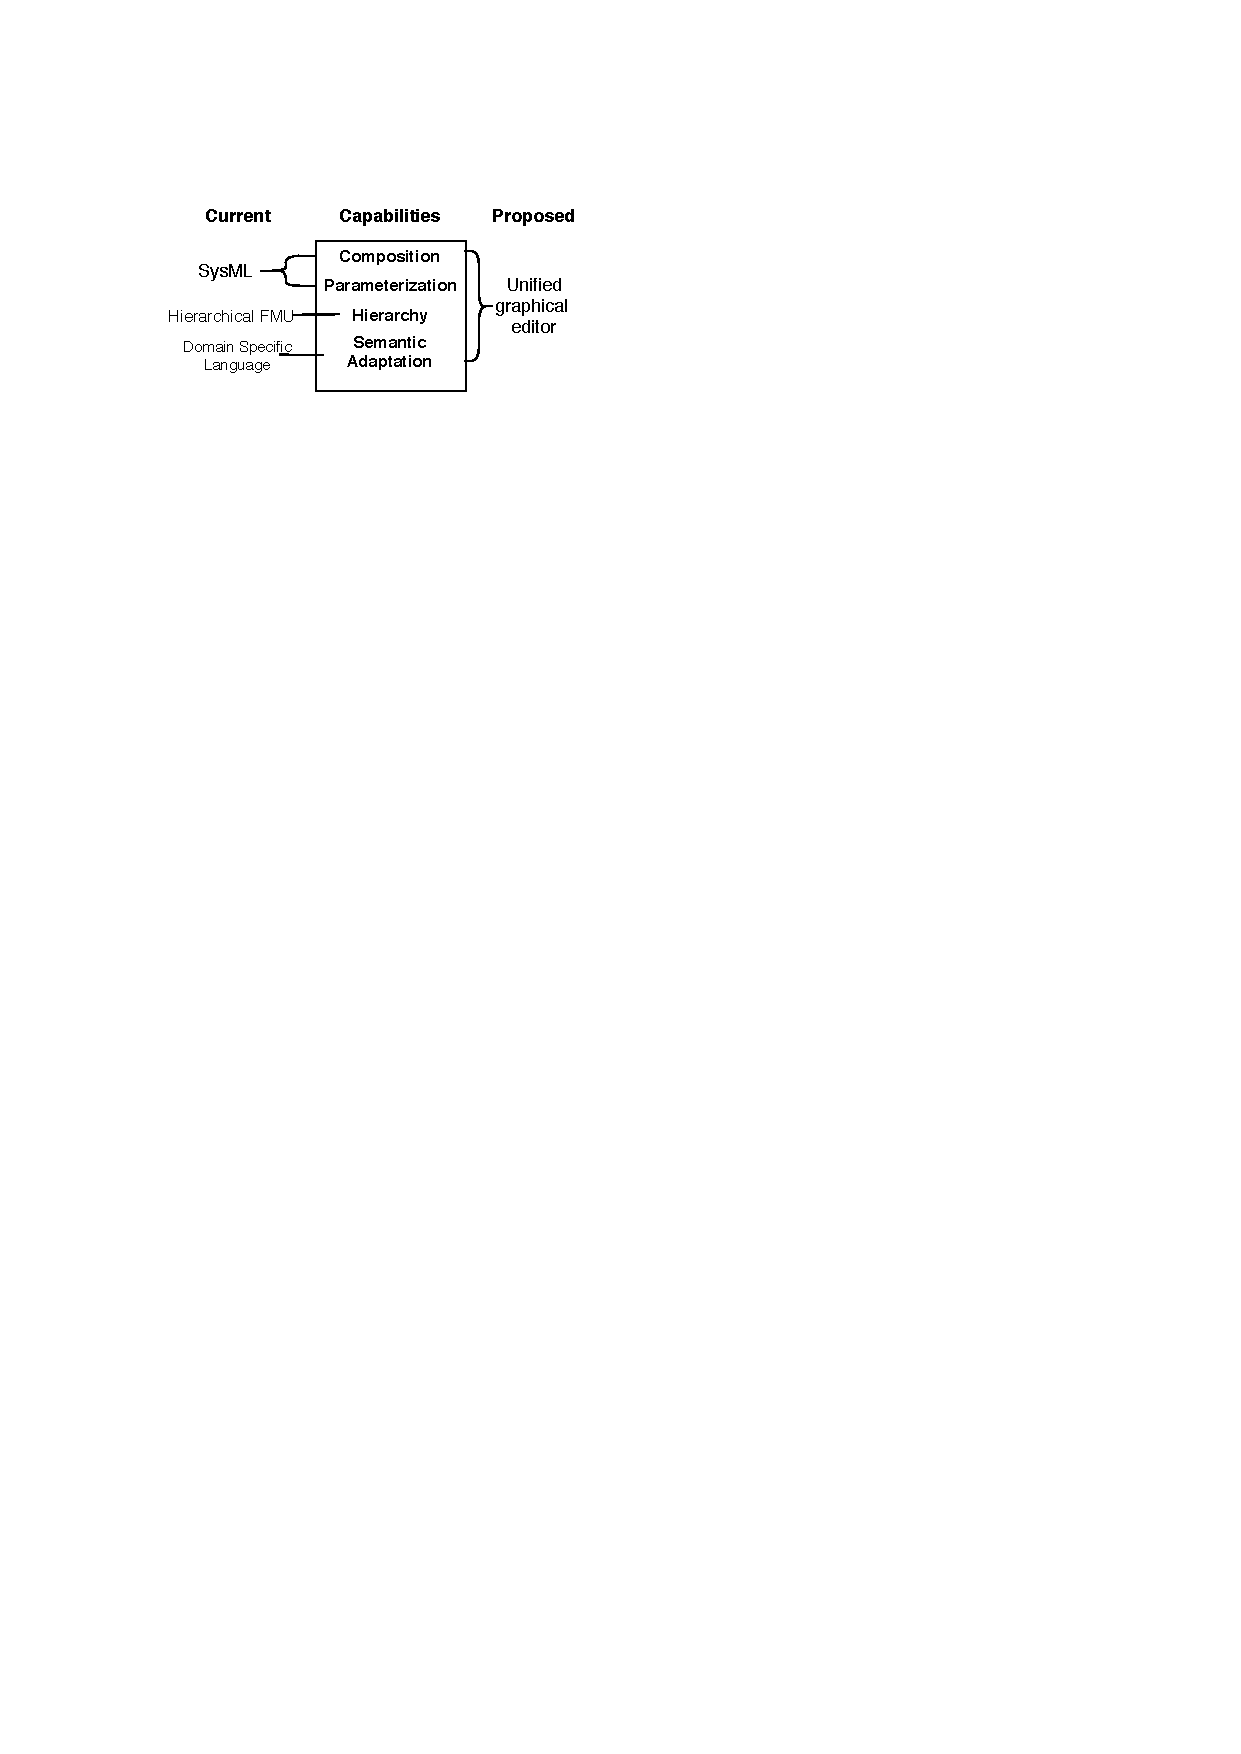
\includegraphics[width=0.8\columnwidth]{Images/technologies.pdf}
\caption{The migration from current capabilities to the proposed graphical solution/representation.}
\label{fig:technologies}
\end{figure}



%\info{It might make sense to refer to tools used in control, electrical circuit, digital design(FPGA) and lab experiments. Specifically one could refer to OMEdit, Simulink, Multisim, Xilinx Vivado and finally NI Lab View.
%These tools have widespread use and their graphical nature supports the arguments in this article.}


The rest of this paper starts with background information for the reader in Section~\ref{sec:background}. Afterwards Section~\ref{sec:intocps} illustrates how the graphical connections are made directly inside the INTO-CPS Application. Then Section~\ref{sec:architecture} provides an introduction to the overall design of the graphical editor. Finally, Section~\ref{sec:conclude} provides a few concluding remarks while Section~\ref{sec:future} provides the future directions expected for this work.